\documentclass[10pt]{book}

\usepackage[pdftex]{graphicx} % with the driver option
\usepackage{amsfonts} 
\usepackage{amsmath} 

\title{Deep Learning for scientists in a hurry. A pedestrian view on Neural Networks for Scientific Applications}
\author{Guillermo Avenda\~no Franco}

\begin{document}
\maketitle
\tableofcontents

\chapter*{Preface}

Deep Learning has revolutionized many aspects of our lives. Being invisible hidden behind our cellphones and computers, Deep Learning is what allows those machines to recognized our voice, organize our photos and over time will be involved in many more aspects of our economy, government and public and private spaces.

% Target audience
This text is an exploration of Deep Learning from the point of view of a scientist. Which can of scientific problems can be solve with Deep Learning? 
It is also a fast and very practical review of the area. The purpose of the book is not to serve Computer Scientist or programmers interested in a comprehensive review of the area. I am not sure if that is actually possible. Maybe CS practitioners can see my book as useful but you are definitely not my target audience. I wrote this book thinking about people with some scientific background but not particular experience in Software Development, Algorithms or GPU programming. 

% Reqs
I assume a rudimentary but effective knowledge of Python scripting. Most of our examples use PyTorch, but we will also demonstrate how to use other popular Deep Learning engines such as TensorFlow and MXNet. At the end what matters is that you know that your scientific questions can have promising answers using Deep Learning techniques and that you can use the tools available to answer those questions.


\chapter{Introduction}

Deep Learning is a powerful tool for solving certain problems that seemed unsolvable just two decades ago. 
The area is also abundant in terminology that if not properly defined could lead to expectations more in the real of science fiction than something that could be accomplish in the nearest future.

Deep Learning is a subject of the larger domain of Machine Learning.
Machine Learning itself is just one of the topics on the even larger Artificial Intelligence area. 
Figure \ref{fig:ai-ml-dl} captures the relations between these subjects. The sizes of the frames has no meaning about the extension of the continent or the content. 

Words like Intelligence, Learning, Neural Network and even the word "deep" could be misleading if we are not careful with definitions and boundaries, separating the science from the fiction.
Lets begin with Artificial Intelligence and pelling out the shell until we arrive to Deep Learning.

\begin{center}
\begin{figure}
\includegraphics[width=\textwidth]{AI-ML-DL.pdf}
\caption{Artificial Intelligence}
\label{fig:ai-ml-dl}
\end{figure}
\end{center}

\section{Artificial Intelligence}

Artificial Intelligence (AI) is charged with immense amount of hype.
People think about AI as the design of sentient robots, robots that will outperform humans in basically all aspects, that will be in appearance indistinguishable from us. AI awakes both hope and fear. 
From the literary point of view they are powerful vehicles to interrogate us about the meaning of being human, our possibilities and limitations. 
Science Fiction writers such as Isaac Asimov and others wrote abundantly about robots, not all of them humanoid in appearance but in many cases very human in their expression, their virtues and flaws. 
Cinema is not less abundant in examples, from the classical Metropolis to recent highly successful Hollywood movies.

Artificial Intelligence is actually more broad and many times more on the earth. 
It is an effort to recreate on a machine intellectual activities naturally performed by humans.
I have chosen carefully all this terms. 
We are talking about recreation, which is not the same as imitation.
Machines today are build very differently from human brains.
A simple imitation will just try fill them mold, to trick us into a copy of what humans do. 
Recreation on the other side is to give new life to how machines carry activities using our brains as inspiration or encouragement but not as its goal.

One of the iconic problems in AI was to produce programs capable of playing chess or go. Two iconic games for which humans were considered until a few years ago unbeatable. 
The first programs were codes with hard-coded rules written by programmers. The code will basically do tree searches exploring possible moves and the consequences of those moves. More advanced programs even stored encyclopedic collections of historic games to serve as databases of game patterns than could be used. 
None of those efforts qualifies on what we will next define as Machine Learning. 
They were, however, explorations on how to create a code that beat humans in an activity for which humans develop procedures and ``intuitions" that allow them to explore a more restrictive set of alternatives. It is clear that humans and machines are approaching the problem from very different angles.

The dominant paradigm of Artificial Intelligence since AI was born back in the 1950s was the idea of encoding "knowledge" as long sets of explicit rules and programming the computer to connect those rules in the form of logical propositions. This is known as \textit{symbolic AI} resulting in the \textit{expert systems} during the 1980s.

A fresh approached emerge with Machine Learning that abandon the explicit coding of rules and concentrating on the effort of creating programs that use examples instead of those rules.

\section{Machine Learning}

Computers are basically the grandsons of looms. In fact before computers were general calculators, people programmed looms to make fabric. 



\chapter{Fundamental Concepts}

The math needed to understand Deep Learning Models is relatively basic.
In this chapter, we start developing the main ideas to understand how neural networks operate. 
We will start with the concept of function, and a perceptron as a simple function and build from it a network of perceptron which is how neural networks are build. 

Central to how neural networks operate are the concept of training a neural network.
Training a neural network consists on adjusting the the parameters that define the network guiding those changes. 
For that we need to define a loss function and a method to induce the changes to the parameters, the back propagation.

We all these elements clear we are ready to understand how to build deep learning models and on the next chapter we will do that using Deep Learning engines such as PyTorch, TensorFlow and MXNet.

A Deep Learning model is a mathematical structure build as network of functions. 
A function is simply a mapping from elements in one set into elements of another set. 
The elements on the first set are called independent variables and the set itself is called the "domain" of the function.
The elements on the destination set are called dependent variables and the set is called the codomain.
Here we are restricting the discussion to cases were both the domain and codomain are not the empty set.

There are many ways of representing a function.
You can tabulate the elements on a table, with a graph with arrows connecting the independent variables with the dependent ones, or with an equation. 
   
For our purpose it is convenient to familiarize with a graphical representation that commonly used later on to build neural networks.
On the figure \ref{fig:monovaluated} we see represented a function.
We interpret the function on this figure from left to right.
One element $x$ is took from  certain domain, for example a real number. 
The function $f()$ will take the element and return another element.
The mapping could be also a real number, but in general a function can return elements from a different set, for example returning integers, colors, labels, etc.

\begin{center}
\begin{figure}
\includegraphics[width=\textwidth]{monovaluated_function.pdf}
\caption{Monovaluated function}
\label{fig:monovaluated}
\end{figure}
\end{center}

A function can return the same element for two different independent variables, but there is only one map from elements on the domain, ie the function can only return one element for each element on the domain.

Functions can take elements from one set or multiple sets. 
A function that takes one single value is called monovaluated, on figure \ref{fig:monovaluated}, $x$ is a single value and the resulting $f(x)$ is also a single value.

One example of a mathematical function for a straight line.
The equation is

$$y = kx + b$$, 

where $k$ is the slope and $b$ the intercept. 

Functions does not need to be lines, functions are not necessarily smooth or even continuous. As we will see later on this chapter, the continuity and smoothness helps the algorithmic treatment of this functions in the context of neural networks. 
Functions are just mappings and if you have a value $x$ in the domain of the function calling the function will return the corresponding answer which is also a single element.

Lets take this opportunity to present two functions that are important for Deep Learning. The sigmoid and the rectified linear function or ReLU.

The sigmoid is a function whose domain are all Real numbers (denoted by $\mathbb{R}$). 

A sigmoid function is a having a characteristic "S"-shaped curve or sigmoid curve.  
There are several functions that possesses a S-shaped behavior. 
A common example of a sigmoid function is the logistic function defined by the formula:

$$S(x) = \frac{1}{1 + e^{-x}} = \frac{e^x}{e^x + 1}=1-S(-x)$$

This is by no means the only possibility. There are similar curves that have a similar appearance.
Many natural processes can be modeled with sigmoids.
One example are learning curves in some complex processes, it exhibits a progression from small beginnings, a process of little return at first that progresses accelerates at some point and approaches a climax slowly over time with small gaining over time. When a specific mathematical model is lacking, a sigmoid function is often used as a suitable representation.

Another function of interest for us is the rectified linear function or ReLU.
It is a function that returns zero for all negative values and returns the the same $x$ for positive values. 
The figure \ref{fig:sigmoid_relu} shows those two functions.

\begin{center}
\begin{figure}
\includegraphics[width=\textwidth]{Sigmoid+ReLU.pdf}
\caption{Sigmoid and ReLU functions}
\label{fig:sigmoid_relu}
\end{figure}
\end{center}

Functions can take more than one value.
In the figure \ref{fig:multivaluated} we see represented a function that takes three values, $x_1$, $x_2$ and $x_3$ and returns a single value mapped as $f(x_1,x_2, x_3)$.
The three values can be arranged as a vector $\vec{x}$ so the function can be written as $f(\vec{x})$.

\begin{center}
\begin{figure}
\includegraphics[width=\textwidth]{multivaluated_function.pdf}
\caption{Multivaluated function}
\label{fig:multivaluated}
\end{figure}
\end{center}

Functions like \ref{fig:multivaluated} are very general. 
There is a particularly simple case for a multivaluated function. 
A linear mapping as shown on \ref{fig:perceptron}. 

\begin{center}
\begin{figure}
\includegraphics[width=\textwidth]{perceptron.pdf}
\caption{Perceptron}
\label{fig:perceptron}
\end{figure}
\end{center}

Take each value $x_i$ and scale it by the factor $w_i$ and add the partial contributions and add a final value $b$. 
The values $w_i$ are called weights and the value $b$ is called the bias.
This particular function has the advantage of simplicity.
It is just a weighted sum of the inputs with the addition of an extra bias.
The bias itself can be included in the set of weights if we consider it as a weight for an additional input that is always 1. 
Doing that we rename $b$ into $w_0$ and now we have a multivaluated function representing a weighted sum of input values.

\begin{equation}
f(\vec{x}) = \sum_{i=0}^n w_i x_i 
\label{eq:linear_model}
\end{equation}

On equation \ref{eq:linear_model} the inputs are the set $\{x_i\}$ with $x_0 = 1$. We have $N+1$ weights with $w_0$ being the bias. 




\begin{center}
\begin{figure}
\includegraphics[width=\textwidth]{multiperceptron.pdf}
\caption{Several Perceptrons}
\end{figure}
\end{center}


Originally conceived as a hardware device, in the modern vision, the perceptron is an algorithm for learning a binary classifier called a Linear classifier, a function that maps its input $\vec{x}$ (a real-valued vector) to an output value $f(\vec{x})$ (a binary return of 0 or 1):


\[
f(\mathbf{x}) = \begin{cases}
1 & \text{if }\ \mathbf{w} \cdot \mathbf{x} + b > 0,\\0 & \text{otherwise}
\end{cases}
\]




\begin{center}
\begin{figure}
\includegraphics[width=\textwidth]{neural_network.pdf}
\caption{Artificial Intelligence}
\end{figure}
\end{center}






\chapter{Three Deep Learning Engines}

Twenty years ago, practitioners of Deep Learning must code their own applications directly on compiled languages such as C or Fortran. 
As the area evolved, Deep Learning engines were developed making easier the creation, exploration and release of new model for production.
Those engines now use high level programming languages such Python, lowering the bar for newcomers and opening oportunities for building models with very little effort.

\section{TensoFLow}

\section{PyTorch}

\section{MXNet}







\end{document}
